\chapter{الضوء ينتشر في خطوط مستقيمة}\label{ch:g4:light-straight-lines}

تميل أشعّة الشمس عبر ضباب الصباح بين الأشجار --- مستقيمة كخيوط
مشدودة، كلها. \omterm{def:g3:first-electric-circuit:bulb}{ومصباح} يدوي في عليّة مغبرّة يلقي نصلًا من \omterm{def:g1:light-and-shadows:source}{ضوء} حادّ
الحافة. وتستطيع أن تسمع صديقًا يناديك من وراء الزاوية، لكنك لا
\emph{تراه} هناك. وهذا كله قانون واحد في ثياب مختلفة --- أقدم
قوانين \omterm{def:g1:light-and-shadows:source}{الضوء}.

\section{قانون الخطّ المستقيم}

\begin{proposition}[الضوء ينتشر في خطوط مستقيمة]\label{prop:g4:light-straight-lines:law}
ينتشر \omterm{def:g1:light-and-shadows:source}{الضوء} في \omterm{def:g2:air-around-us:air}{الهواء} (كما في الماء والزجاج والفضاء الخالي) في
خطوط مستقيمة. فهو لا ينعطف حول الزوايا، ولا يهيم مثل الدخان،
ولا ينثني ليجدك خلف جدار. وحيث لا يبلغ خطّ مستقيم من المنبع لا
يصل \omterm{def:g1:light-and-shadows:source}{ضوء} من ذلك المنبع.
\end{proposition}

\begin{definition}[الشعاع الضوئي]\label{def:g4:light-straight-lines:ray}
لرسم \omterm{def:g1:light-and-shadows:source}{الضوء} يستعمل الفيزيائيون \emph{الشعاع
الضوئي}\index{شعاع ضوئي}: خطًّا مستقيمًا عليه سهم، يبيّن خيطًا
واحدًا من \omterm{def:g1:light-and-shadows:source}{الضوء} والجهة التي يجري فيها. فحزمة \omterm{def:g3:first-electric-circuit:bulb}{المصباح} اليدوي
تُرسم مروحة من أشعّة؛ وحزمة الليزر الرفيعة تُرسم شعاعًا واحدًا.
والشعاع، مثل سهم \omterm{def:g2:pushes-and-pulls:force}{القوة}، رسم صغير يحمل في داخله قانونًا: أن طرق
\omterm{def:g1:light-and-shadows:source}{الضوء} مستقيمة كالمسطرة.
\end{definition}

\begin{omfigure}
\begin{tikzpicture}[scale=0.85]
  \draw[thick, fill=omExo, fill opacity=0.3]
    (0.2,1.3) rectangle (1.4,2.3);
  \draw[thick] (1.4,1.45) -- (1.4,2.15);
  \draw[-Stealth, omThm, thick] (1.4,2.1) -- (10.6,2.9);
  \draw[-Stealth, omThm, thick] (1.4,1.8) -- (10.6,1.8);
  \draw[-Stealth, omThm, thick] (1.4,1.5) -- (10.6,0.7);
  \node[below, font=\small] at (0.8,1.1) {مصباح يدوي};
  \node[above, font=\small] at (6.0,2.75)
    {مروحة من أشعّة: كل واحد منها مستقيم كالمسطرة};
\end{tikzpicture}

{\small حزمة \omterm{def:g3:first-electric-circuit:bulb}{مصباح} يدوي مرسومة على طريقة الفيزيائيين: أشعّة
مستقيمة، عليها أسهم تبيّن جهة جريان \omterm{def:g1:light-and-shadows:source}{الضوء}.}
\end{omfigure}

\begin{example}[أين يُظهر القانون نفسه]\label{ex:g4:light-straight-lines:sightings}
متى عرفت القانون رأيته في كل مكان: في أشعّة الشمس المستقيمة عبر
الضباب أو المصاريع؛ وفي الحافة المستقيمة الحادّة لحزمة \omterm{def:g3:first-electric-circuit:bulb}{مصباح}
يدوي في \omterm{def:g2:air-around-us:air}{هواء} مغبرّ؛ وفي خيط مؤشّر الليزر المستقيم استقامة تامّة؛
وفي كل منارة تكنس بنصال \omterm{def:g1:light-and-shadows:source}{ضوء} مستقيمة بحرَ الليل. أما \omterm{def:g1:light-and-shadows:source}{الضوء}
المنثني فلا يُرى أبدًا --- قد تنحني النافورات والغابات، أما
\omterm{def:g1:light-and-shadows:source}{الضوء} فلا.
\end{example}

\begin{omfigure}
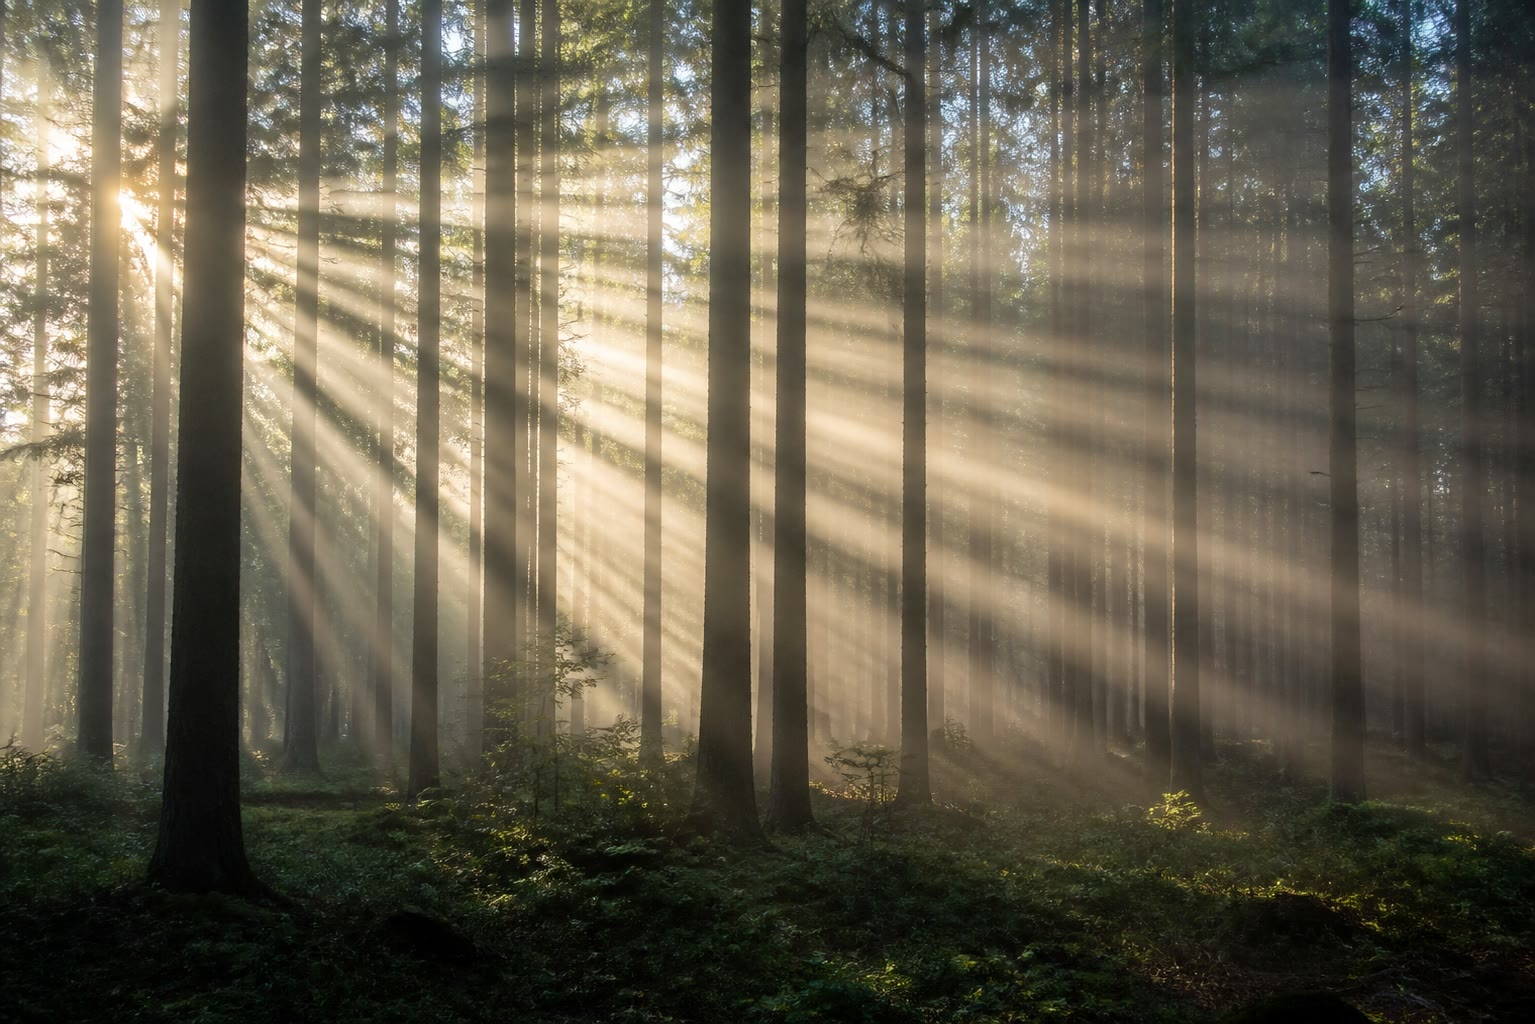
\includegraphics[width=0.58\linewidth]{images/book1/ai/g4-light-sunbeams.jpg}

{\small برهان الطبيعة نفسها: أشعّة الشمس عابرةً هواءً ضبابيًّا مستقيمة استقامة تامّة --- \omterm{def:g1:light-and-shadows:source}{فالضوء} لا ينثني حول الأشجار.}
\end{omfigure}

\section{برهان بثلاث بطاقات}

\begin{method}[تجربة البطاقات الثلاث]\label{met:g4:light-straight-lines:cards}
\begin{enumerate}
  \item اثقب ثقبًا صغيرًا في وسط ثلاث بطاقات قاسية، على الارتفاع
        نفسه؛
  \item وانصب البطاقات قائمة في صفّ، بينها شبر، وشمعة مشتعلة (أو
        \omterm{def:g3:first-electric-circuit:bulb}{مصباح} يدوي) وراء آخرها؛
  \item وحرّك رأسك حتى ترى اللهب عبر الثقوب الثلاثة --- ولا
        يمكن ذلك إلا حين تقف الثقوب الثلاثة واللهب على خطّ
        مستقيم واحد (وتحقّق: فخيط مشدود عبر الثقوب يبلغ اللهب)؛
  \item ثم أزلق البطاقة الوسطى جانبًا، بمقدار عرض إصبع فقط.
\end{enumerate}
فيختفي اللهب. \omterm{def:g1:light-and-shadows:source}{والضوء} الذي كان في وسعه أن يتعرّج --- عبر الثقب
الأول، ثم قفزة جانبية، ثم عبر الثقب المزاح، ثم إلى عينك ---
لا يفعل ذلك ببساطة: فلا خطّ مستقيم، فلا \omterm{def:g1:light-and-shadows:source}{ضوء}.
\end{method}

\begin{omfigure}
\begin{tikzpicture}[scale=0.85]
  \draw[thick] (1.0,0.3) -- (1.0,2.5) (3.6,0.3) -- (3.6,2.5)
    (6.2,0.3) -- (6.2,2.5);
  \fill[white] (0.92,1.32) rectangle (1.08,1.48);
  \draw[thick] (0.92,1.32) rectangle (1.08,1.48);
  \fill[white] (3.52,1.32) rectangle (3.68,1.48);
  \draw[thick] (3.52,1.32) rectangle (3.68,1.48);
  \fill[white] (6.12,1.32) rectangle (6.28,1.48);
  \draw[thick] (6.12,1.32) rectangle (6.28,1.48);
  % a real candle: wax body, wick, teardrop flame
  \draw[thick, fill=yellow!15] (8.42,0.3) rectangle (8.78,1.02);
  \draw[thick] (8.6,1.02) -- (8.6,1.16);
  \draw[thick, orange!80!red, fill=yellow!80]
    (8.6,1.16) .. controls (8.44,1.3) and (8.47,1.47) .. (8.6,1.58)
    .. controls (8.73,1.47) and (8.76,1.3) .. (8.6,1.16);
  \fill[orange!90] (8.6,1.27) ellipse (0.045 and 0.08);
  % the ray of light, dead straight through the three holes
  \draw[-Stealth, line width=1.3pt, yellow!75!orange]
    (8.44,1.4) -- (-0.4,1.4);
  \node[below, font=\small] at (8.6,0.05) {شمعة};
  \node[below, font=\small] at (-0.2,1.2) {عين};
  \node[above, font=\small] at (4.6,2.55)
    {ثلاثة ثقوب على خطّ مستقيم واحد: فيُرى اللهب};
\end{tikzpicture}

{\small تجربة البطاقات الثلاث: يُرى اللهب بالضبط حين يصطفّ
اللهب والثقوب والعين على استقامة واحدة. أزِح بطاقة واحدة، فيموت
المنظر.}
\end{omfigure}

\begin{example}[الظلال وقد فُسّرت إلى الأبد]\label{ex:g4:light-straight-lines:shadows}
الآن يسلّم \omterm{def:g1:light-and-shadows:shadow}{ظلّ} سنتك المدرسية الأولى سرّه. فالأشعّة تجري مستقيمة
من \omterm{def:g3:first-electric-circuit:bulb}{المصباح}؛ والكرة توقف ما يصطدم بها منها؛ والأشعّة التي تخطئ
حافّتها بالكاد تواصل جريانها مستقيمة. وخلف الكرة يقع بالضبط
الحيّز الذي لا يبلغه شعاع مستقيم --- وهو \omterm{def:g1:light-and-shadows:shadow}{الظلّ}، وحافّته الحادّة
رسمتها آخر الأشعّة انسلالًا. فأشعّة مستقيمة وظلال حادّة: ولو
كان \omterm{def:g1:light-and-shadows:source}{الضوء} معوجًّا لطمس كل \omterm{def:g1:light-and-shadows:shadow}{ظلّ} في ضباب.
\end{example}

\section{الرؤية استقبال للضوء}

\begin{proposition}[كيف تعمل الرؤية]\label{prop:g4:light-straight-lines:seeing}
ترى الشيء حين ينتقل \omterm{def:g1:light-and-shadows:source}{ضوء} منه في خطّ مستقيم إلى عينك --- ضوؤه هو
إن كان منبعًا، وإلا \omterm{def:g1:light-and-shadows:source}{فضوء} شمس أو \omterm{def:g3:first-electric-circuit:bulb}{مصباح} مرتدّ عنه. ولا يخرج من
عينك شيء ليمسك العالَم: فالرؤية \emph{استقبال}، والتقاط للأشعّة
كما تلتقط شبكةٌ كراتٍ.
\end{proposition}

\begin{example}[من وراء الزاوية]\label{ex:g4:light-straight-lines:corner}
ينادي صديقك من وراء زاوية المدرسة: فتسمعه ولا تستطيع أن تراه.
\omterm{def:g3:sound-around-us:sound}{فالصوت} ينتشر مثل حلقات البركة ويلتفّ حول حافة الزاوية؛ أما
\omterm{def:g1:light-and-shadows:source}{الضوء} فيتمسّك بطرقه المستقيمة، ولا خطّ مستقيم يصل وجه صديقك
بعينك عبر الآجرّ. ولكي ترى من وراء الزوايا لا بدّ أن \emph{تطوي
الطريق} --- أن تعطي الشعاع سطحًا قاسيًا لامعًا يرتدّ عنه. وتلك
الحيلة تُسمّى المرآة، ولها أول فصل ضوئي في السنة القادمة.
\end{example}

\begin{remark}[العدّاء البطل]\label{rem:g4:light-straight-lines:speed}
\omterm{def:g3:sound-around-us:sound}{الصوت}، كما قسنا، يهرول \qty{340}{m} في كل ثانية. أما \omterm{def:g1:light-and-shadows:source}{الضوء} على
طرقه المستقيمة ففي دوري آخر تمامًا: إذ يعبر السماء كلها أسرع
ممّا يستطيع عدّ أن يلحقه --- ولهذا تصل الومضة ``في الحال''
ويتثاقل الرعد وراءها بثوانٍ. فكم سرعته بالضبط؟ العدد من الشناعة
بحيث ندّخره لسنة لاحقة --- مع حكاية الحيل البارعة التي لزمت
لقياسه أصلًا.
\end{remark}

\section{تمارين}

\begin{exercise}[$\star$]\label{exo:g4:light-straight-lines:1}
اذكر قانون هذا الفصل. وسمِّ مشهدين تراه فيهما في الخارج.
\end{exercise}

\begin{exercise}[$\star$]\label{exo:g4:light-straight-lines:2}
ما \omterm{def:g4:light-straight-lines:ray}{الشعاع الضوئي}، وأيّ شيئين يبيّنهما رسمه؟
\end{exercise}

\begin{exercise}[$\star$]\label{exo:g4:light-straight-lines:3}
في تجربة البطاقات الثلاث، متى تستطيع أن ترى اللهب بالضبط؟ وأيّ
حركة واحدة تُخفيه، ولماذا؟
\end{exercise}

\begin{exercise}[$\star$]\label{exo:g4:light-straight-lines:4}
كيف يفسّر قانون الخطّ المستقيم حدّةَ حافة \omterm{def:g1:light-and-shadows:shadow}{الظلّ}؟
\end{exercise}

\begin{exercise}[$\star$]\label{exo:g4:light-straight-lines:5}
أنت ترى هذا الكتاب الآن. احكِ رحلة \omterm{def:g1:light-and-shadows:source}{الضوء} التي تجعل ذلك ممكنًا،
من \omterm{def:g3:first-electric-circuit:bulb}{مصباح} إلى عينك.
\end{exercise}

\begin{exercise}[$\star$]\label{exo:g4:light-straight-lines:6}
لماذا تسمع صديقًا من وراء الزاوية ولا تراه؟ وماذا يفعل كل
مسافر --- \omterm{def:g3:sound-around-us:sound}{الصوت} \omterm{def:g1:light-and-shadows:source}{والضوء} --- عند الزاوية؟
\end{exercise}

\begin{exercise}[$\star$]\label{exo:g4:light-straight-lines:7}
ثقب مفتاح، وغرفة مضاءة وراءه، وعينك: فمن أيّ مواضع الممرّ
المظلم تستطيع أن ترى \omterm{def:g3:first-electric-circuit:bulb}{المصباح} عبر ثقب المفتاح؟ أجب بخطّ
مستقيم.
\end{exercise}

\begin{exercise}[$\star$]\label{exo:g4:light-straight-lines:8}
أيّهما يصل أولًا من ألعاب نارية بعيدة، الدويّ أم الومضة؟ وأيّ
قانون وأيّ \omterm{def:g2:measuring-length:measure}{قياس} من هذه السنة يفسّر الفجوة؟
\end{exercise}

\begin{exercise}[$\star$]\label{exo:g4:light-straight-lines:9}
``حين أنظر إلى \omterm{def:g4:solar-system:star}{نجم} ينطلق شيء من عيني ليلمسه.'' صحّح هذا الاعتقاد
القديم بما في \cref{prop:g4:light-straight-lines:seeing} ---
ما الذي ينتقل، وفي أيّ جهة؟
\end{exercise}

\begin{exercise}[$\star\star$]\label{exo:g4:light-straight-lines:10}
صمّم، برسم للأشعّة، طريقة لمراقبة الممرّ من داخل غرفتك بحيلة
المرآة الملمَّح إليها في
\cref{ex:g4:light-straight-lines:corner}: أين يجب أن يقف السطح
اللامع عند المدخل، وماذا يفعل بطريق الشعاع؟ (والغوّاصات تستعمل
هذا بعينه، مرتين إحداهما فوق الأخرى، لترى فوق الأمواج.)
\end{exercise}

\begin{exercise}[$\star\star$]\label{exo:g4:light-straight-lines:11}
في صباح ضبابي تتفتّح أشعّة الشمس بين الأشجار في خطوط مستقيمة
ظاهرة --- ومع ذلك يقول صديقك: ``نحن نرى الأشعّة، فلا بدّ أن
\omterm{def:g1:light-and-shadows:source}{الضوء} مادة مرئية معلّقة في \omterm{def:g2:air-around-us:air}{الهواء}.'' فما الذي ترونه في الحقيقة
حين تظهر ``حزمة'' في الضباب أو الغبار، وكيف تبدو الحزمة في \omterm{def:g2:air-around-us:air}{هواء}
نظيف تمامًا؟
\end{exercise}
